Nous avons évoqué les menaces qui pesaient sur les interfaces nord et sud, mais il existe encore d'autres menaces :

\begin{itemize}

\item Sur le contrôleur en lui même : bien que cela soit laborieux et que je n'aie pas réussi à le faire durant mon stage, il n'est pas impossible qu'il existe des vulnérabilités dans le code source du contrôleur. Sans aller jusqu'à l'exécution de code arbitraire (sachant que le code est en Java, donc cela nécessite normalement une faille de la machine virtuelle, puisqu'à aucun endroit du code la possibilité est offerte d'exécuter du code externe si on supprime le cas d'une application externe), il est envisageable de trouver des enchaînements (mise à jour de variables bien choisies, modification de l'état interne du contrôleur) qui réalisent des actions non prévues. Cela demande cependant une connaissance excellente du code, ce qu'il est très compliqué d'obtenir vu le peu de documentation qui est offerte lorsqu'on souhaite se plonger dans le coeur du contrôleur et la complexité générale de l'ensemble.\\

Sur le contrôleur on peut aussi trouver un problème de répudiation : bien que les logs soient sauvegardés et soient assez complets, rien n'empêche à l'heure actuelle de les supprimer (le but étant plus de fournir du debug au développeur qu'un outil d'analyse forensique voire une preuve certaine des évènements passés).\\

Enfin toujours sur le contrôleur, on peut trouver des problèmes de DoS, comme par exemple en 2015 avec la CVE-2015-7516\footnote{https://wiki.onosproject.org/display/ONOS/Security+advisories}. Cela revient là encore à utiliser les faiblesses du code pour avoir une action non prévue néfaste sur les performances globales.\\

\item Sur les échanges inter-contrôleurs : le concept SDN prévoit la possibilité de gestion à plusieurs contrôleurs du réseau SDN. Pour cela, il est nécessaire que les contrôleurs partagent entre eux la topologie à laquelle ils ont accès. Cela introduit une vulnérabilité supplémentaire puisque sans authentification mutuelle, il existe un risque de parler à un contrôleur malveillant envoyant de fausses informations.\\

\item Sur les stations d'administration et de déploiement : comme sur un réseau classique, si on compromet les machines utilisées pour gérer le réseau ou distribuer les mises à jour logicielles (social engineering, compromission de l'environnement (DNS ou ARP spoofing, ...)), on a théoriquement un accès privilégié au contrôleur (selon les modes d'authentification utilisés) qui permet donc sans y être autorisé d'y apporter des modifications importantes.\\

\item Sur les éléments du réseau : bien que cela demeure peu probable, les mêmes attaques que sur un réseau classique sont toujours possibles. Elles permettent ensuite d'utiliser les attaques sur l'API southbound.

\end{itemize}

Le très récent site regroupant entre autres les projets Security-mode ONOS, Delta et Barista \footnote{http://sdnsecurity.org} (nous en reparlerons dans la conclusion) nous donne un bon récapitulatif d'une partie des attaques que nous allons détailler et qui s'inscrivent dans les catégories précédentes :
\begin{figure}[h]
  	\centering
  	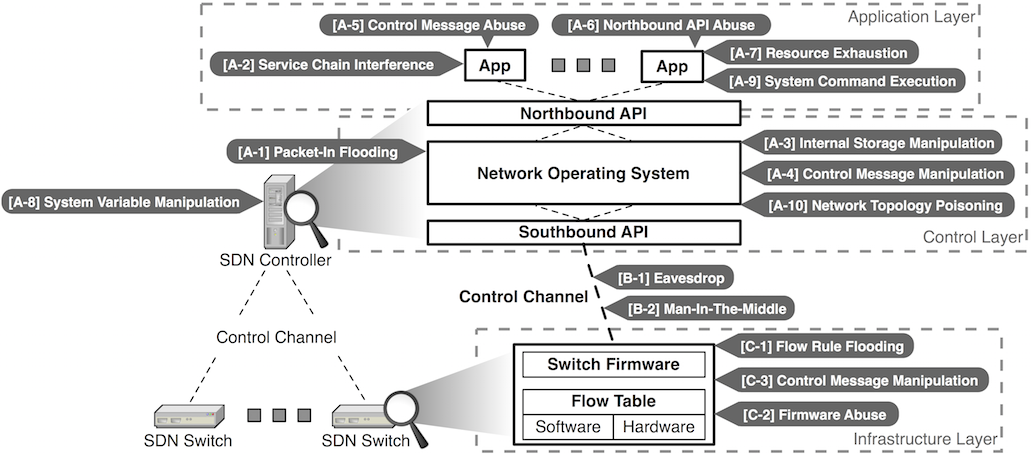
\includegraphics[width=1\textwidth]{threats.png}
  	\caption{Principales menaces sur un réseau SDN}
\end{figure}
